\documentclass[11pt,a4paper]{article}

\usepackage[T1]{fontenc}
\usepackage[utf8]{inputenc}
\usepackage{lmodern}
\usepackage[english]{babel}
\usepackage{microtype}
\usepackage[margin=2.3cm]{geometry}
\usepackage{amsmath}
\usepackage{graphicx}
\usepackage{float}
\usepackage{booktabs}
\usepackage{tabularx}
\usepackage{array}
\usepackage{xcolor}
\usepackage{enumitem}
\usepackage{caption}
\usepackage{tikz}
\usetikzlibrary{arrows.meta,positioning}
\usepackage[hidelinks]{hyperref}

\graphicspath{{images/}}
\setlength{\parindent}{0pt}
\setlength{\emergencystretch}{3em}
\setlength{\parskip}{5pt plus 2pt}
\setlist{itemsep=1pt,topsep=3pt}
\captionsetup{font=small,labelfont=bf}
\newcolumntype{Y}{>{\raggedright\arraybackslash}X}
\newcommand{\code}[1]{\texttt{\small #1}}
\definecolor{accent}{HTML}{1F6FEB}

\tikzset{
  box/.style={draw=accent,rounded corners=2pt,fill=accent!8,minimum height=7mm,minimum width=24mm,align=center,font=\small},
  core/.style={box,draw=black,fill=black!8,font=\small\bfseries},
  arr/.style={-{Stealth[length=2.2mm]},thick,draw=black!70}
}

\title{\textbf{QuantBacktest}\\[2pt]\large Financial Strategy Backtesting Platform}
\author{Alexandre Tung \and Victor Haegeman \and Eloi Dumas \and Alexis Launay-Schapman\\[4pt]
\small EFREI Paris, ST2OOS, 2026/2027}
\date{\small Source code: \url{https://github.com/Alexarmanto/QuantBacktest-Financial-Strategy-Backtesting-Platform}}

\begin{document}
\maketitle

\section{Introduction}

A backtest answers one question: if I had followed this trading rule in the past, what would have happened to my money? We built a backtesting website in C\# (.NET 10, ASP.NET Core MVC) that fetches prices from the Alpha Vantage API, keeps them locally, simulates trading strategies on daily and weekly data, measures their performance and generates reports. The user interface is shown in the demonstration video, so this report focuses on design choices and results.

The application covers every requirement of the subject, with 10 strategies and a buy \& hold baseline where 6 were asked for. We added features that make a result easier to trust: stop-loss, take-profit, trailing stop and slippage; an optimisation heatmap with an overfitting warning; train/test validation; a strategy comparator; Monte Carlo simulation; a data quality panel; a no-code strategy builder; permanent links; and a Docker image.

\begin{table}[H]
\centering\small
\begin{tabularx}{\textwidth}{lY}
\toprule
\textbf{Member} & \textbf{Responsibility} \\
\midrule
Alexandre Tung & Alpha Vantage client, SQLite cache, data quality, PDF and CSV reports, Docker \\
Victor Haegeman & Indicators, strategies, no-code rule engine, Monte Carlo \\
Eloi Dumas & Backtesting engine, advanced orders, metrics, optimisation heatmap \\
Alexis Launay-Schapman & Web application, comparator, train/test, permanent links \\
\bottomrule
\end{tabularx}
\caption{Split of the work.}
\end{table}

\section{Architecture}

With four people working at the same time, our priority was to avoid blocking each other. The solution has one shared project, \code{Core}, and one project per responsibility (Figure~\ref{fig:layers}). \code{Core} only contains interfaces, data models and constants. What a signature cannot say, such as the price at which an order is filled, is written in a contract with numbered rules (X1--X15 for execution, M1--M14 for metrics, D1--D8 for data\dots) that the code and the tests quote. We froze this contract early and never had to change it.

\begin{figure}[H]
\centering
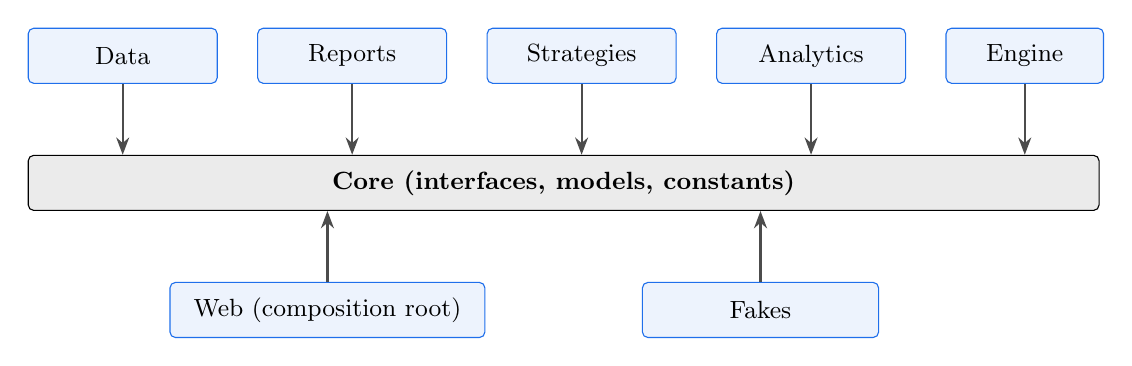
\begin{tikzpicture}[node distance=6mm and 5mm]
\node[core,minimum width=136mm] (core) {Core (interfaces, models, constants)};
\node[box,above=9mm of core.north west,anchor=south west] (data) {Data};
\node[box,right=of data] (reports) {Reports};
\node[box,right=of reports] (strategies) {Strategies};
\node[box,right=of strategies] (analytics) {Analytics};
\node[box,right=of analytics,minimum width=20mm] (engine) {Engine};
\node[box,below=9mm of core.south,minimum width=40mm,xshift=-30mm] (web) {Web (composition root)};
\node[box,below=9mm of core.south,minimum width=30mm,xshift=25mm] (fakes) {Fakes};
\foreach \n in {data,reports,strategies,analytics,engine} \draw[arr] (\n.south) -- (\n.south |- core.north);
\draw[arr] (web.north) -- (web.north |- core.south);
\draw[arr] (fakes.north) -- (fakes.north |- core.south);
\end{tikzpicture}
\caption{Every project depends on \code{Core} only. \code{Web} also references the others, only to plug them in.}
\label{fig:layers}
\end{figure}

A project never references the project of another part: parts communicate through interfaces injected by dependency injection. For a backtest, the web layer calls \code{IBacktestService}, which gets the strategy from \code{IStrategyCatalog} and the prices from \code{IMarketDataService}, then runs \code{IBacktestEngine}. The resulting \code{BacktestResult} is displayed and is the input of the Monte Carlo service and of the report generator. A \code{Fakes} project implements every interface, so the web pages could be built before the real engine existed; one setting per part switches between the fake and the real service.

Some conventions removed whole families of bugs: \code{decimal} for money and \code{double} for statistics; fractions in the code and percentages only on screen; invariant culture for parsing; an injected clock; and \code{null} (shown as ``n/a'') for an undefined ratio, never \code{NaN} or 0.

\section{Data layer}

\textbf{What the free plan gives.} We first tested the endpoints with a free key. The full daily history and the adjusted daily series are premium: we only get the last 100 raw daily bars. The adjusted weekly series, however, is free and goes back to 1999 (1,406 bars), so long tests use weekly data.

\textbf{Cache and seed files.} Prices are stored in SQLite with EF Core. Without a refresh, the cache is returned with no API call, so a backtest is reproducible. If the cache is empty, a committed seed file is imported (AAPL, MSFT, SPY, JPM), or else the API is called. A refresh merges bars by date and never deletes one; if it fails, the cache is unchanged. Seed files also let the application run without a key.

\textbf{Pitfalls of the API.} The project guide gave a good starting point, but we met three traps. Alpha Vantage reports errors as JSON with HTTP 200, so testing the status code would save an error message as data: our client detects and classifies these answers. \code{double.Parse("123.45")} without a culture misreads the number on a French system, so we always use the invariant culture, and a test runs under \code{fr-FR}. Finally, the key is in the URL and even in the rate limit message of the API: it is only read from user-secrets or an environment variable, our messages never copy the API text, and HTTP logging is removed. After a real refresh in Docker, the key did not appear anywhere in the logs.

\textbf{Quota and concurrency.} The 25 daily requests are counted per UTC day before sending, so failures count too. Simultaneous calls for a series share one download: 10 calls send one HTTP request.

\textbf{Data quality.} A report computed on cached data flags price jumps above 25\,\%, zero volumes, five identical closes in a row, and calendar gaps. It finds real events (Figure~\ref{fig:quality}): the 11-day gap of September 2001 and the violent moves of JPM during the 2008 crisis. A flag is an invitation to look, not necessarily an error.

\begin{figure}[H]
\centering
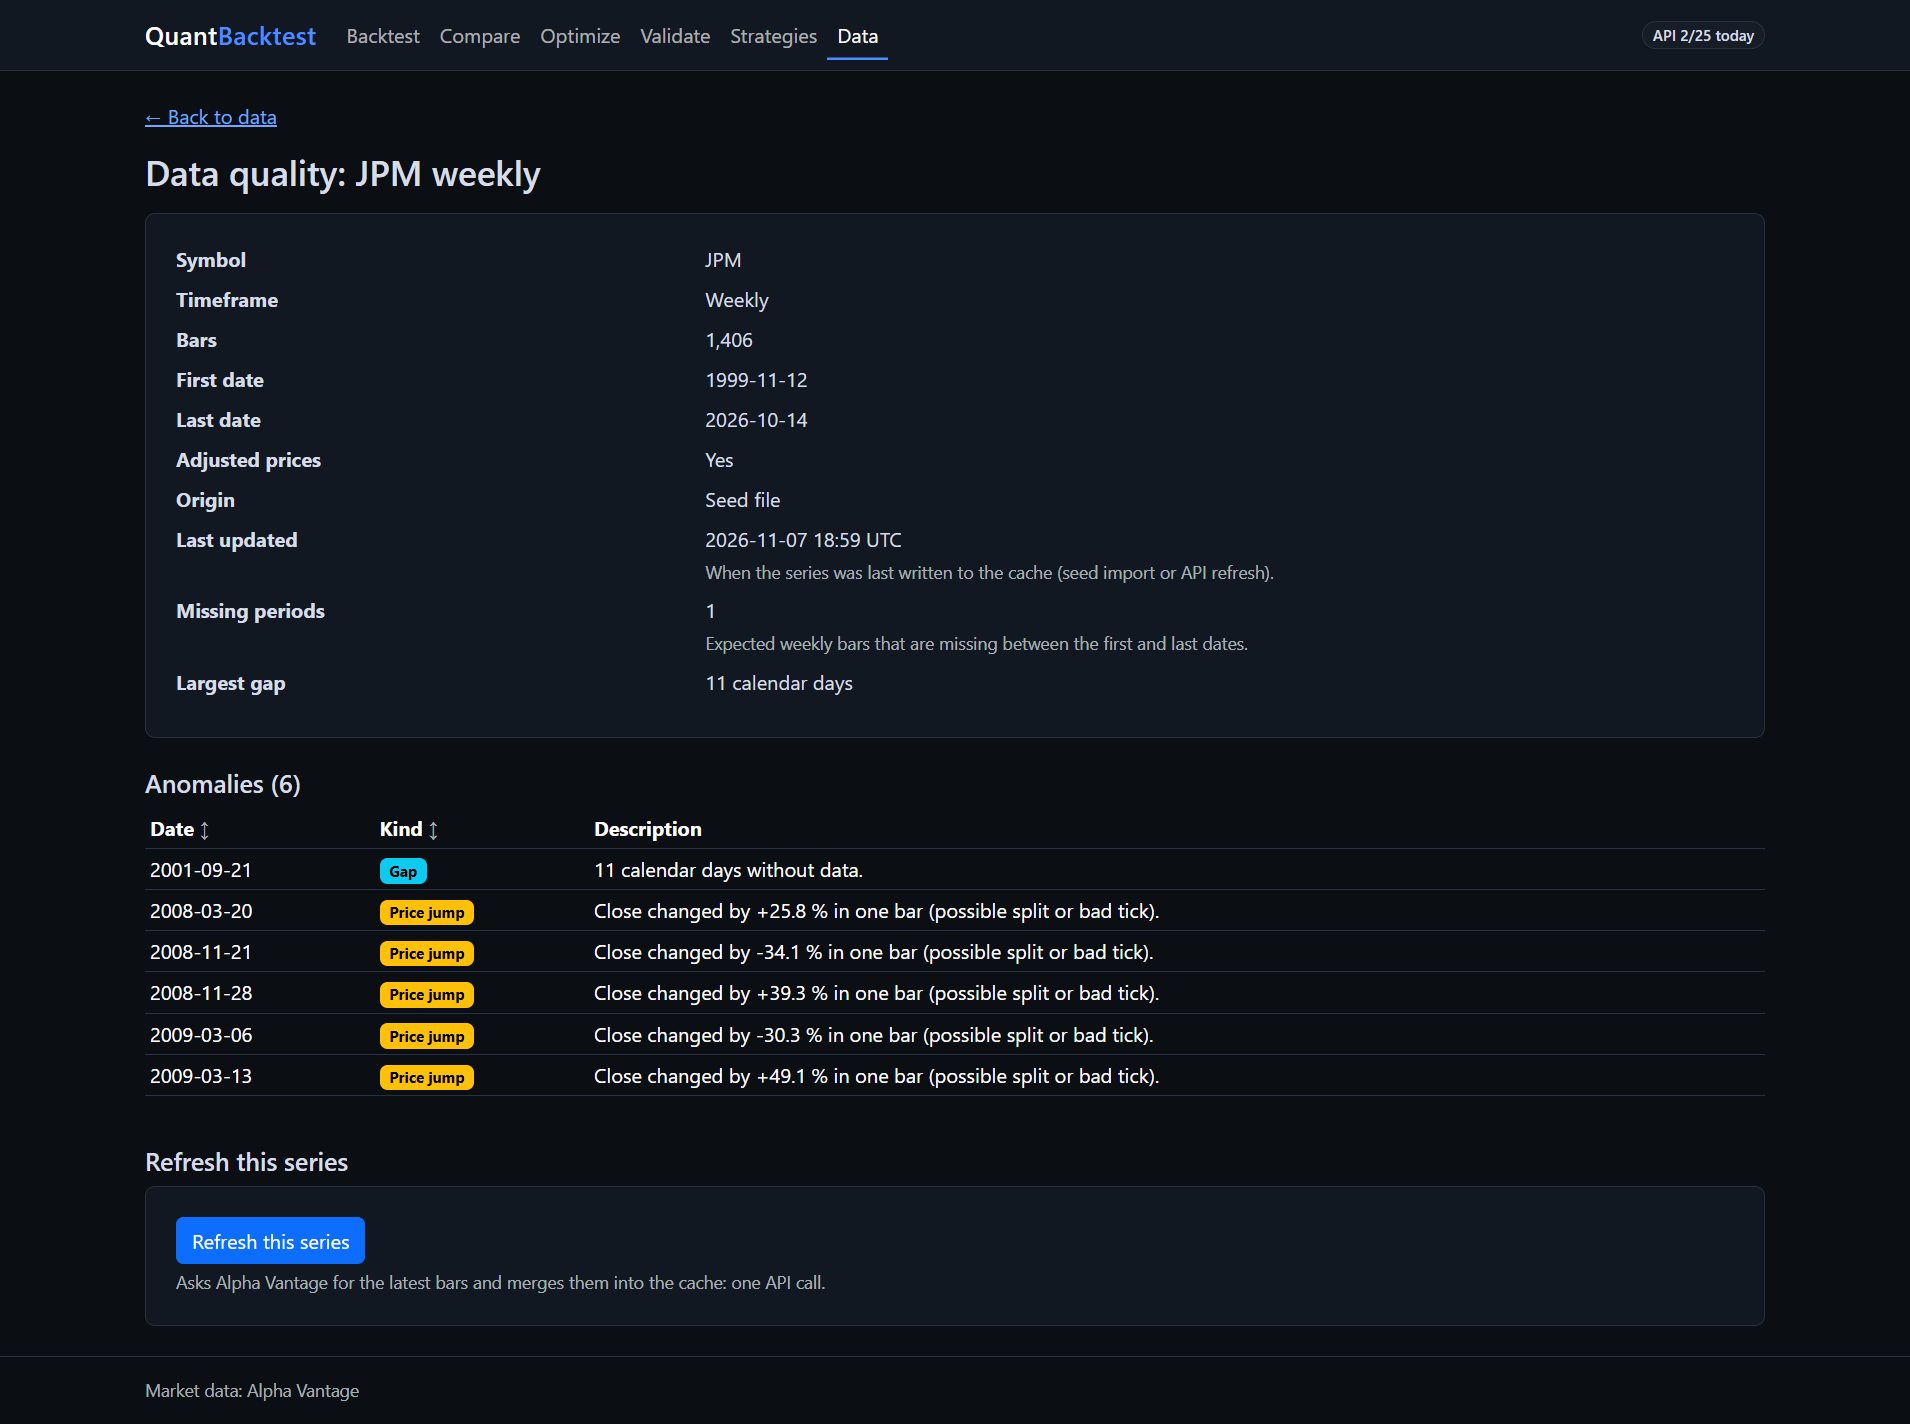
\includegraphics[width=0.68\textwidth]{part4-12-data-quality-detail.png}
\caption{Quality report of JPM weekly: one gap and five price jumps.}
\label{fig:quality}
\end{figure}

\section{Strategies}

A strategy only returns \code{Buy}, \code{Sell} or \code{Hold} for each bar, and knows nothing about capital, fees or stops. It is deterministic and may only use past bars. All strategies share one implementation of the indicators (SMA, EMA, Bollinger, RSI, ROC, MACD, highest high and lowest low). Classes are discovered by reflection, so adding one does not touch the web project; a commented C\# template makes this easy.

Users can also build strategies without code: an entry and an exit rule, each with 1 to 5 conditions combining prices, volume, constants and indicators. A definition is validated, stored as JSON, and becomes a normal strategy.

Table~\ref{tab:spy} shows the strategies on SPY weekly from 1999 to 2026, with default parameters and a 0.1\,\% fee. Turn of the month accepts daily data only and is absent.

\begin{table}[H]
\centering\small
\begin{tabular}{lrrrrr}
\toprule
\textbf{Strategy} & \textbf{Return} & \textbf{Sharpe} & \textbf{Max drawdown} & \textbf{Trades} & \textbf{Exposure} \\
\midrule
Moving average crossover & +759.4\,\% & 0.70 & 31.8\,\% & 9 & 70.9\,\% \\
Donchian breakout & +300.9\,\% & 0.57 & 27.9\,\% & 22 & 61.0\,\% \\
Buy and hold & +781.5\,\% & 0.55 & 54.6\,\% & 1 & 99.9\,\% \\
Momentum (ROC) & +258.5\,\% & 0.48 & 38.5\,\% & 68 & 68.7\,\% \\
Trend-filtered RSI-2 & +111.7\,\% & 0.40 & 23.5\,\% & 42 & 9.2\,\% \\
RSI reversion & +156.9\,\% & 0.37 & 43.4\,\% & 4 & 20.6\,\% \\
MACD crossover & +94.0\,\% & 0.29 & 40.9\,\% & 59 & 53.3\,\% \\
Bollinger + RSI & +56.6\,\% & 0.24 & 37.4\,\% & 6 & 5.0\,\% \\
Bollinger reversion & +67.7\,\% & 0.23 & 41.4\,\% & 20 & 14.2\,\% \\
Consecutive down days & +30.0\,\% & 0.17 & 39.8\,\% & 57 & 7.3\,\% \\
\bottomrule
\end{tabular}
\caption{SPY weekly, 1,406 bars, default parameters, sorted by Sharpe ratio.}
\label{tab:spy}
\end{table}

Only the moving average crossover comes close to buy \& hold, with a much smaller drawdown because it stays out of long declines. Mean reversion strategies are rarely invested on weekly bars, which explains their low returns. Many results rest on very few trades, so this table alone does not prove that one strategy is better.

\section{Backtesting engine}

\textbf{Execution.} A signal is computed at the close of a bar and executed at the \textbf{Open of the next bar}, so it cannot use a price that did not exist yet. Positions are long only and use all the cash. With a slippage $s$ and a fee $f$, a buy is filled at $p(1+s)$, with quantity $q = \text{cash}/(\text{fill}(1+f))$, and a sale at $p(1-s)$, with proceeds $q\,\text{fill}\,(1-f)$. Bars before the requested period only warm up the indicators.

\textbf{Protective exits.} The stop level is the highest of $E(1-\text{SL})$ and $\text{peak}(1-\text{TS})$, and the target is $E(1+\text{TP})$, with $E$ the entry price. If a bar opens beyond a level, the exit is at the Open. If stop and target are both touched in one bar, the order is unknown, so we prudently assume the stop came first.

\textbf{Metrics.} We compute 13 metrics for the strategy and for buy \& hold, including the cumulative and annualized return, volatility, maximum drawdown, win rate, profit factor and exposure. With $P$ periods per year (252 or 52) and $r_t$ the returns:
\[
\text{Sharpe} = \frac{\bar r - r_f}{\sigma(r)}\sqrt{P},\qquad
\text{Sortino} = \frac{\bar r - r_f}{\sqrt{\frac1n\sum\min(0,r_t-r_f)^2}}\sqrt{P},\qquad
\text{Calmar} = \frac{\text{annualized return}}{\text{max drawdown}}.
\]

\textbf{Heatmap.} Up to 625 pairs of parameters go through the same validation and engine as a normal backtest. An optimiser always finds a best cell, even on noise, so a warning appears when the best value is more than twice the average of its neighbours.

\textbf{Checking the numbers.} Expected values in the 184 engine tests are recomputed from the formulas, never copied from the output. Scenarios were also computed independently in a spreadsheet (Figure~\ref{fig:hand}). Property tests on random signals check that the equity is never negative, that the final equity equals the capital plus the profits, and that truncating the future does not change the past.

\begin{figure}[H]
\centering
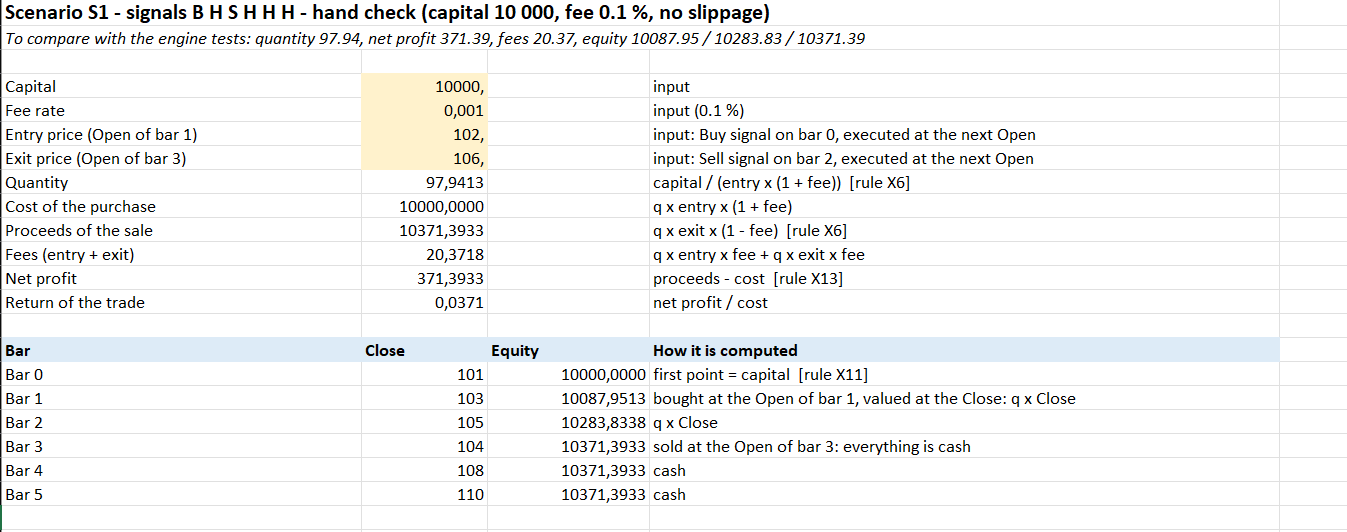
\includegraphics[width=0.72\textwidth]{part3-02-hand-check-spreadsheet.png}
\caption{A six-bar scenario recomputed by hand: quantity, fees, net profit and equity.}
\label{fig:hand}
\end{figure}

\section{Robustness analysis}

A good backtest proves little on its own, so we added two tools.

\textbf{Train/test.} The page optimises on the first part of the period (70\,\% by default) and tests the best parameters once on the rest. On AAPL weekly since 2010, the crossover with fast 26 and slow 35 has a Sharpe ratio of 1.02 in training and 0.75 in test. This drop is expected, since the parameters were chosen on the training data. With 5 and 6 trades, neither figure is statistically solid.

\textbf{Monte Carlo.} We draw the returns of the trades at random with replacement and compound them, 100 to 10,000 times, from a fixed seed. This gives distributions of the final return and of the trade-level drawdown. \textit{Consecutive down days} on AAPL weekly has a 68.7\,\% probability of loss, and its actual result (-41.98\,\%) is near the median: it is simply a losing strategy. The crossover on MSFT weekly has an 8.5\,\% probability of loss, but percentiles ranging from -17.4\,\% (P5) to +29,111\,\% (P95): with 15 trades, one of which earned +521\,\%, the result depends heavily on that single trade.

\section{Web application}

The site has six pages: Backtest, Compare, Optimize, Validate, Strategies and Data. The video shows them in use. The web project contains no financial logic: controllers call the services and view models format the values. Forms and strategy cards are generated from the catalog, so no strategy is hard-coded. Only the exceptions of the contract are shown to the user, with the input kept; anything else is a bug and reaches a generic error page. Every result has a \code{GET} URL holding all its settings, and one class writes a single canonical form of it, so a result can be shared and reproduced. Bootstrap and Chart.js are served locally.

\begin{figure}[H]
\centering
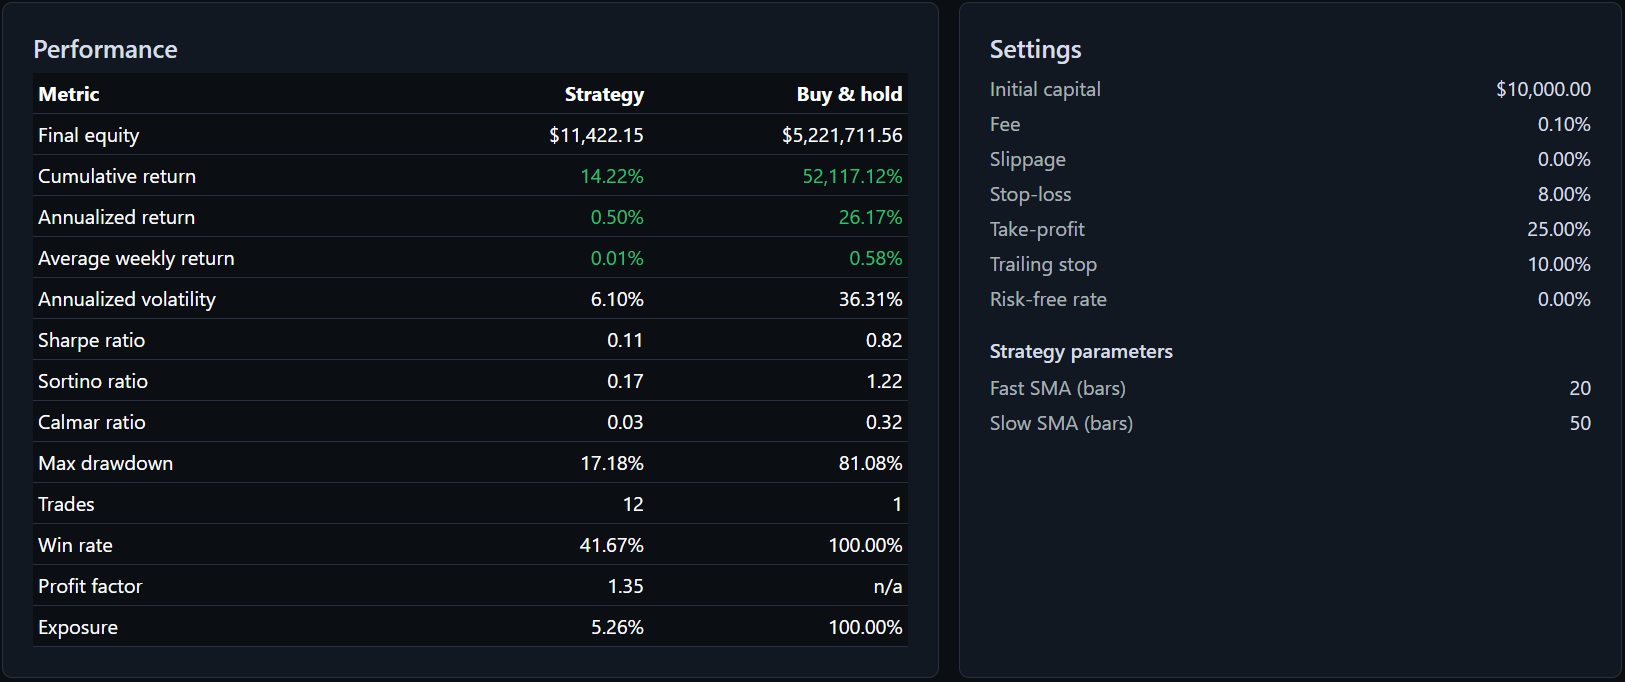
\includegraphics[width=0.8\textwidth]{report-real-metrics.png}
\caption{Results of a real backtest: AAPL weekly, moving average crossover with stops.}
\end{figure}

\section{Reports and deployment}

The PDF report is built with QuestPDF and ScottPlot (Figure~\ref{fig:pdf}). Every number comes from \code{BacktestResult} and nothing is recomputed, so the report cannot disagree with the screen. We checked one real report by hand: for MSFT weekly, the 15 net profits add up to 85,964.29, which matches the printed final equity of 95,964.29. Trades can also be exported as CSV.

\begin{figure}[H]
\centering
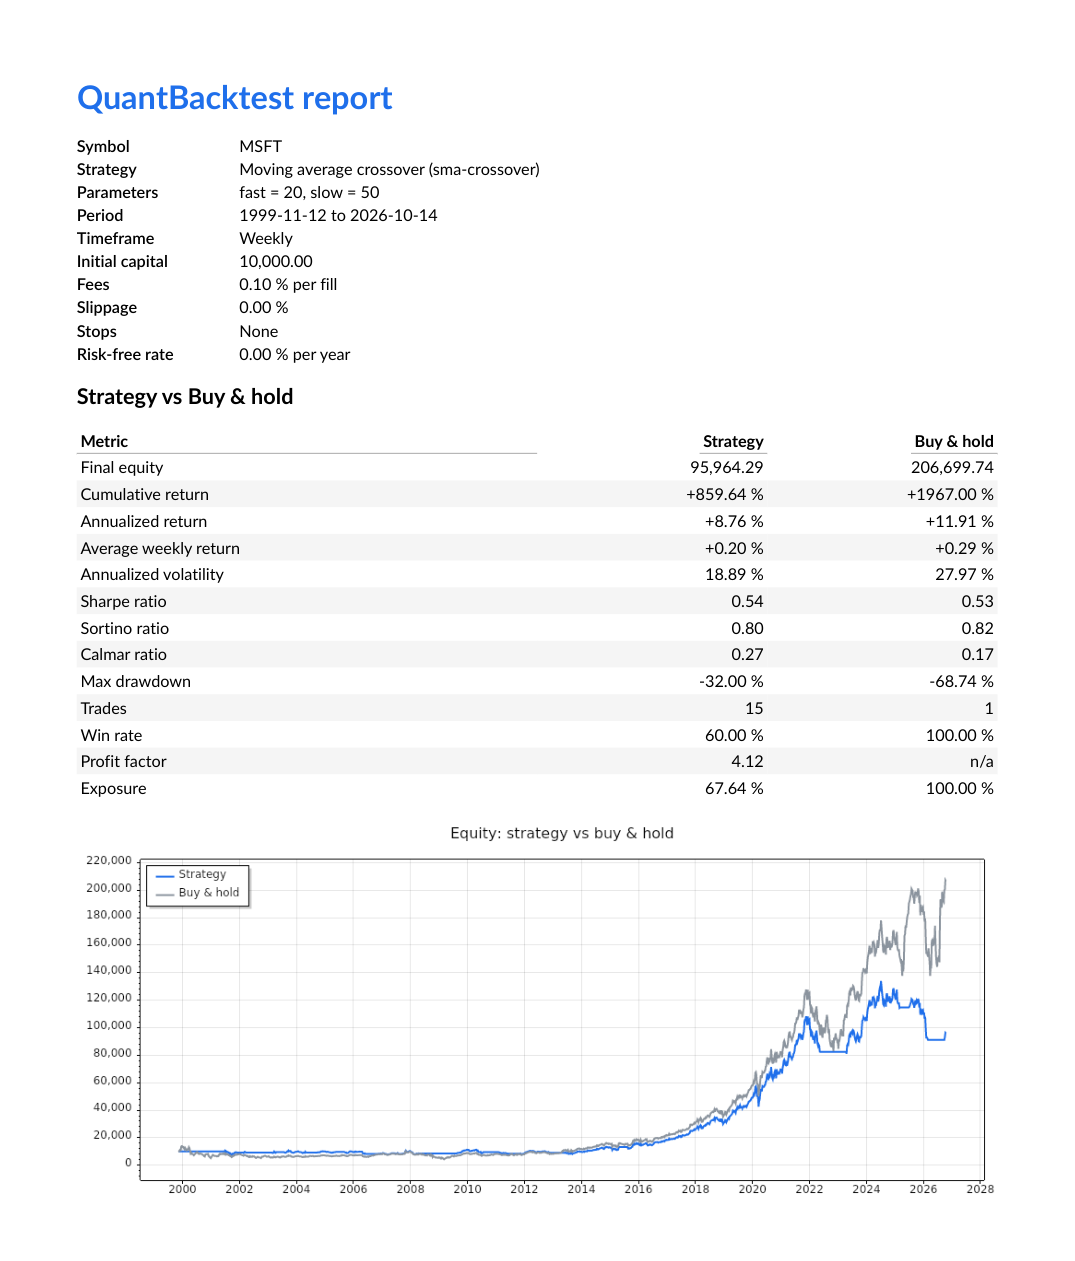
\includegraphics[height=7.2cm]{part1-08-pdf-page1.png}\hspace{4mm}
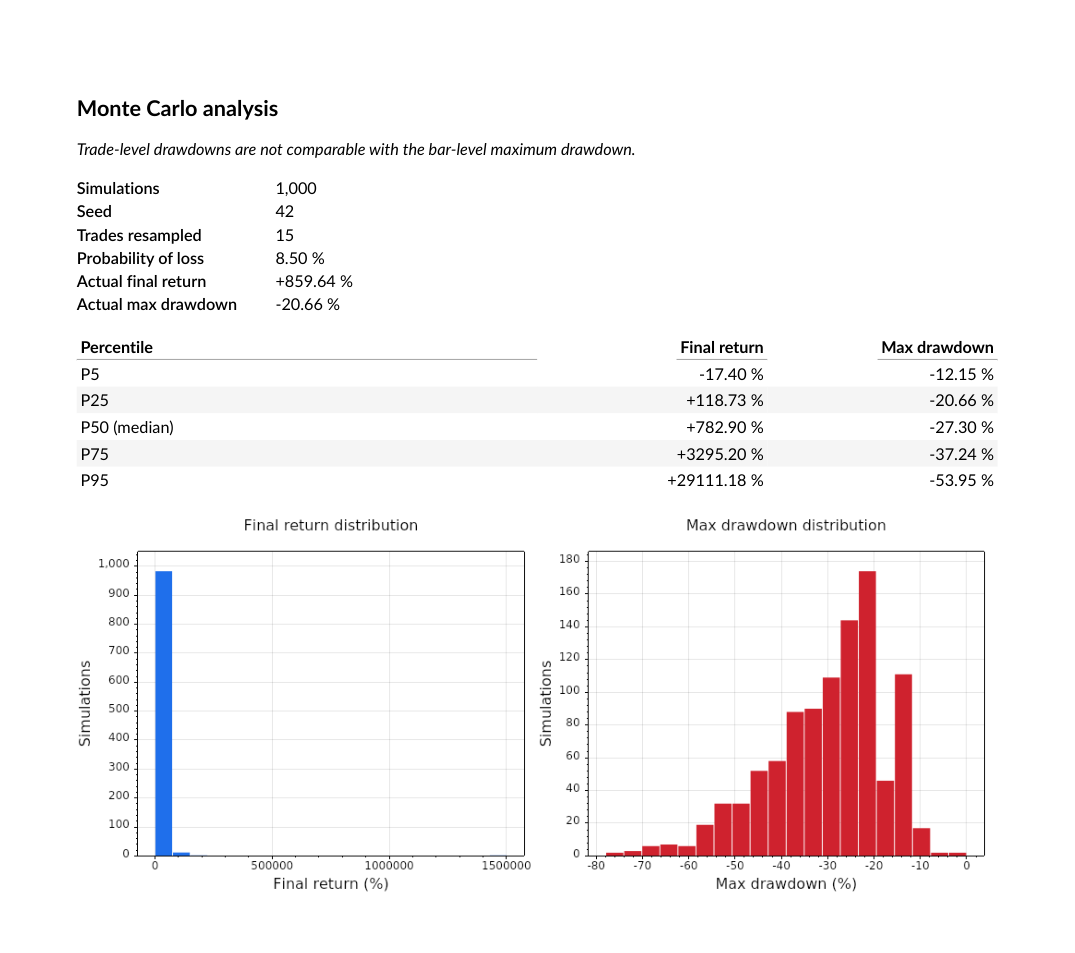
\includegraphics[height=7.2cm]{part1-12-pdf-montecarlo.png}
\caption{PDF report: summary page and Monte Carlo page.}
\label{fig:pdf}
\end{figure}

\code{docker compose up --build} starts the application on port 8080. The image is only built if the solution compiles with warnings as errors and all the tests pass. It runs as a non-root user, keeps the database in a named volume and reads the API key from a local \code{.env} file that is never committed. We ran it with Docker Desktop, including a real API refresh and the generation of a PDF.

\section{Quality and teamwork}

The solution has 1,494 automated tests with no network and no real clock: Web 923, Engine 184, Strategies 168, Data 124, Reports 55, Analytics 14, Fakes 14, Core 12. Each test quotes the rule it checks. Razor views, JavaScript and CSS were checked by hand.

All changes went through pull requests, on branches named after each part: 42 were merged between 13 October and 8 November 2026. GitHub Actions compiles with warnings as errors, runs all tests, checks the title of the pull request and verifies that the changed files belong to the part of the branch. Branch protection requires these checks and forbids force-pushes. We removed the mandatory approval on 15 October because it slowed us down, while keeping it for contract changes; the CI cannot replace a human reading the code, so this was a compromise.

Our most useful decision was to write a precise contract before the code. We also learned that a backtest can be wrong in silent ways (a look-ahead, a misread decimal, an error saved as data), which is why the tools showing the limits of a result matter as much as the strategies.

\section{Limitations and future work}

\begin{itemize}
\item \textbf{Data.} Only 100 raw daily bars are free, so long tests are weekly; seed files are snapshots of October 2026. A paid source would give long adjusted daily histories.
\item \textbf{Simulation.} Long only, no leverage, no volume limit, no taxes and no interest on cash. Inside a bar, the order of the High and the Low is unknown.
\item \textbf{Validation.} Train/test uses a single split, and walk-forward validation would be better. Monte Carlo resamples one backtest and assumes independent trades.
\item \textbf{Interface.} Only the equity chart has a log scale, and the comparator uses default parameters.
\item \textbf{Method.} Our symbols are large, successful companies chosen with hindsight, on which buy \& hold is hard to beat. Past results do not predict future results.
\end{itemize}

\appendix
\section{User manual}

\textbf{Start.} With Docker: copy \code{.env.example} to \code{.env}, optionally add a free Alpha Vantage key, run \code{docker compose up --build} and open \url{http://localhost:8080}. Without Docker: set the key with \code{dotnet user-secrets set "AlphaVantage:ApiKey" "<key>" --project src/QuantBacktest.Web}, then run \code{dotnet run --project src/QuantBacktest.Web} and open \url{http://localhost:5080}. Without a key, AAPL, MSFT, SPY and JPM still work.

\begin{table}[H]
\centering\small
\begin{tabularx}{\textwidth}{lY}
\toprule
\textbf{Page} & \textbf{Use} \\
\midrule
Backtest & Choose a symbol, timeframe, strategy and settings. Empty stops are disabled. The result offers the PDF, the CSV, Monte Carlo and optimisation. \\
Compare & Run 2 to 5 strategies with default parameters on the same data. \\
Optimize & Test pairs of two parameters. An ``isolated peak'' warning suggests overfitting. \\
Validate & Optimise on the first part of the period and test on the rest. \\
Strategies & Read each strategy's rules and risks, and create no-code strategies. \\
Data & See cached series and their quality report, and refresh a series (1 of 25 daily calls). \\
\bottomrule
\end{tabularx}
\end{table}

\textbf{C\# strategy.} Copy \code{Custom/TemplateStrategy.cs} into the \code{Strategies} folder, remove \code{[HiddenStrategy]}, set a unique id, fill in the rules and rebuild.

\textbf{Common messages.} \emph{API key not configured}: set the key, or use a symbol with a seed file. \emph{Request limit reached}: wait for midnight UTC or use cached symbols. \emph{Prices are not adjusted}: normal for daily data; use weekly for long tests. \emph{Not enough trades for Monte Carlo}: at least 5 trades are needed.

\end{document}
